\newcommand{\state}[1]{\texttt{#1}}%
\newcommand{\racing}{\state{Racing}}%
\newcommand{\recovery}{\state{Recovery}}%
\newcommand{\SL}{\state{Straight Line}}%
\newcommand{\C}{\state{Curve}}%
\newcommand{\OT}{\state{Out of Track}}%
\newcommand{\St}{\state{Stuck}}%
\newcommand{\AC}{\state{Approaching Curve}}%
\newcommand{\IT}{\state{Inside Track}}%

\begin{figure*}[t]
\centering
\begin{subfigure}[b]{0.4\textwidth}
	\centering%
	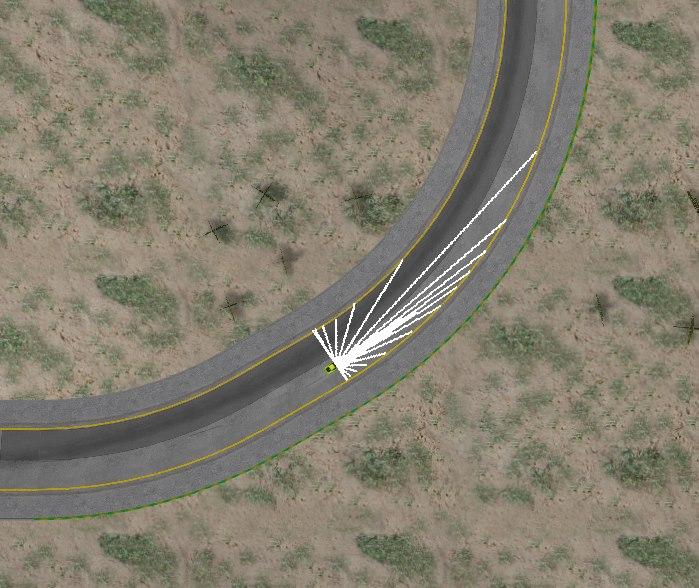
\includegraphics[height=.8\textwidth]{img/FarthestSensor}
	\caption{Sensor input in \C.}\label{fig:FSensor}%
\end{subfigure}\hfill
\begin{subfigure}[b]{0.4\textwidth}
		\centering
		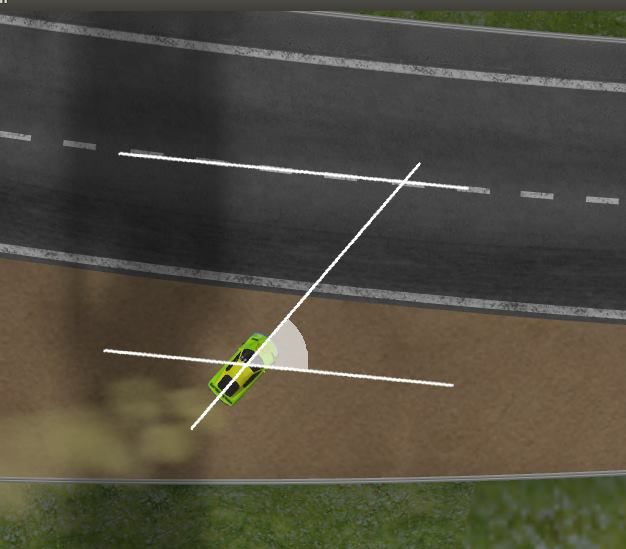
\includegraphics[height=.8\textwidth]{img/ReturnAngle}
		\caption{Angle between car and track axis in \OT.}\label{fig:Angle}%
\end{subfigure}
   \caption{Range finders readings for FSMDriver model.}\label{fig:FSMDriver}
\end{figure*}

\section{FSMDriver}\label{sec:3}%
Driving a car can be intuitively divided into several behaviors, and thus provide a straightforward implementation as a finite-state machine model. Such model's configuration parameters can be optimized through a genetic algorithm, and the TORCS/SCR platform provides a standard measure of driver quality, while its sensor/actuator interface enables it to be readily replaced by actual robotic prototypes (or other more advanced simulators) for further testing. This work proposes to use these ideas for evolving a controller for a car, the FSMDriver, as one more step towards autonomous vehicles.



%%%%%%%%%%%%%%%%%%%%%%%%%%%%%%%%%%%%%%%%%%%%%%%%%%%%%%%%%%%%%%%%%%%%%%%%%%%%%%%%
%%%%%%%%%%%%%%%%%%%%%%%%%%%%%%%%%%%%%%%%%%%%%%%%%%%%%%%%%%%%%%%%%%%%%%%%%%%%%%%%
%%%%%%%%%%%%%%%%%%%%%%%%%%%%%%%%%%%%%%%%%%%%%%%%%%%%%%%%%%%%%%%%%%%%%%%%%%%%%%%%



\subsection{Driving Behaviors}%
A \state{state} in the FSM model considered here defines a racing behavior, deciding the driver's output solely based on the given sensor input (a Moore machine~\cite{Ajzerman}). The FSM implements a transition function that, at every game tick, analyzes the sensor inputs, as defined by SCR's interface, and decides which state best represents the current situation, triggering a change in states if necessary. The current state then processes the sensor readings and defines the proper actuator outputs according to its implementation.

Intuitively, a single \state{Driving} state could be a definite solution for such FSM model, but self-driving cars are obviously involved in several distinct situations, each of which could be translated into a state and, if possible, developed independently from the others. Not only does this approach make it easier to develop and test changes, it also enables parallel implementation.

Considering TORCS/SCR as the testing environment, it is clear that two antagonistic situations which require specific behaviors exist: \racing, for situations where the car is in ``proper'' racing conditions, and \recovery, for when it is in such situation that distinct actions are required to return to the racing conditions. These can be further divided into the more specific behaviors for implementation:
\begin{description}
	\item[\SL:] for racing straight ahead;
	\item[\C:] for racing through a curve;
	\item[\OT:] for recovering from leaving the track or facing the wrong direction; and
	\item[\St:] for recovering from being unable to move forward.
\end{description}

Each of these states implements its racing policies as follows. \SL~ attempts to go as fast as possible parallel to the track axis by accelerating at full throttle, and changing gears according to RPM thresholds. \C~steers towards the direction towards the track sensor with the largest reading (see Figure~\ref{fig:FSensor}) with 60\% throttle, braking in case it starts to slide in the $X$ axis. \OT~ attempts to return to the track, facing the right direction, adjusting its speed and steering according to its current orientation concerning the track (see Figure~\ref{fig:Angle}). \St~tries to get unstuck by using the reverse gear and hard steering for a limited amount of game ticks and then switching to \OT~or a \racing~state.

The transition function for this FSMDriver, presented in Algorithm~\ref{alg:FSMDriver}, is quite intuitive. The car is considered stuck if it can only move in a very slow speed or not at all for some duration, it is considered inside the track by direct sensors reading and in a curve if the readings from the range finders in both sides are not too different.

\begin{algorithm}[!h]%
\caption{FSMDriver Transition}%
\label{alg:FSMDriver}%
\begin{algorithmic}
    \IF{car is stuck}
        \STATE $state \Leftarrow \St$
    \ELSE
		\IF{car is inside track}
			\IF{car is in curve}
				\STATE $state \Leftarrow \C$
			\ELSE
				\STATE $state \Leftarrow \SL$
			\ENDIF
		\ELSE
			\STATE $state \Leftarrow \OT$
		\ENDIF
	\ENDIF
\end{algorithmic}
\end{algorithm}

Initially, random configurations for the states' parameters were set and manually adjusted until an acceptable behavior was achieved, i.e. such a configuration in which a car could successfully complete a race. In the beginning, the \recovery~states (\OT~and \St) were constantly triggered, and therefore were first to be adjusted for improved behavior. Eventually their settings were such that the \racing~behaviors could be focused on. These too were manually and arbitrarily set through trial and error, considering the driver's performance (time and damage) and skill (visual analysis of tests).

After several iterations, this model performed better than some of the less capable robots available in TORCS, showcasing the FSMDriver's potential for controlling a car.



%%%%%%%%%%%%%%%%%%%%%%%%%%%%%%%%%%%%%%%%%%%%%%%%%%%%%%%%%%%%%%%%%%%%%%%%%%%%%%%%
%%%%%%%%%%%%%%%%%%%%%%%%%%%%%%%%%%%%%%%%%%%%%%%%%%%%%%%%%%%%%%%%%%%%%%%%%%%%%%%%
%%%%%%%%%%%%%%%%%%%%%%%%%%%%%%%%%%%%%%%%%%%%%%%%%%%%%%%%%%%%%%%%%%%%%%%%%%%%%%%%



\subsection{FSMDriver5}

\begin{figure*}
\centering
\begin{subfigure}[b]{0.4\textwidth}
   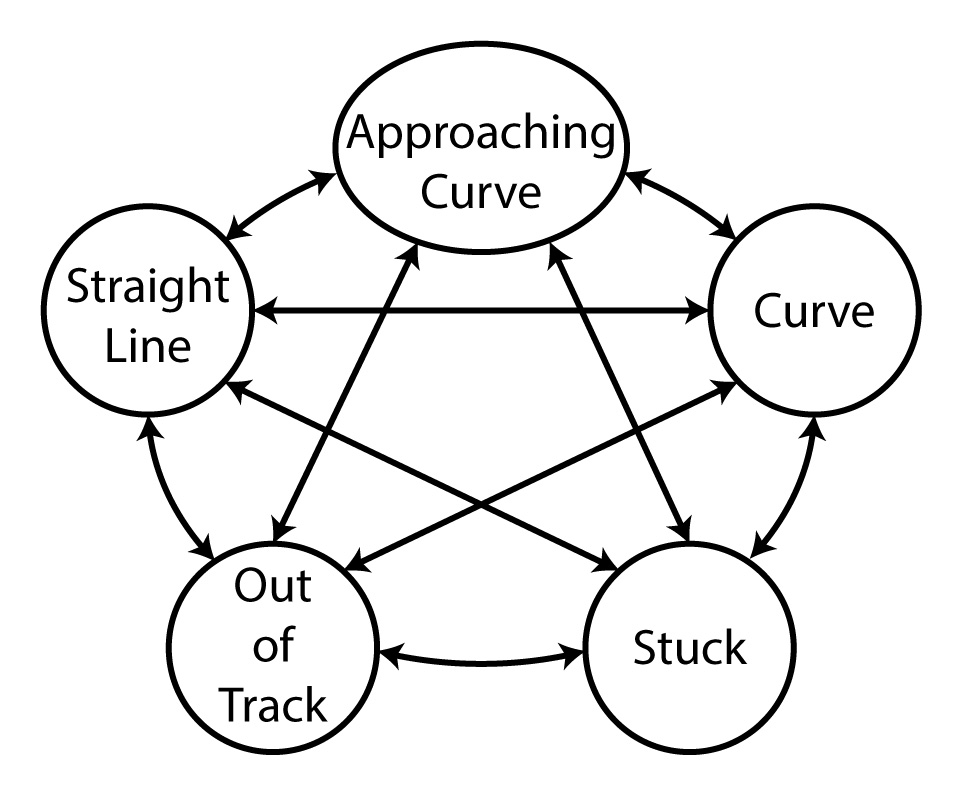
\includegraphics[width=\textwidth]{img/FiveStateFSM}
   \caption{States and transitions.}\label{fig:FSMDriver5Model}%
\end{subfigure}
\hfill
\begin{subfigure}[b]{0.4\textwidth}
   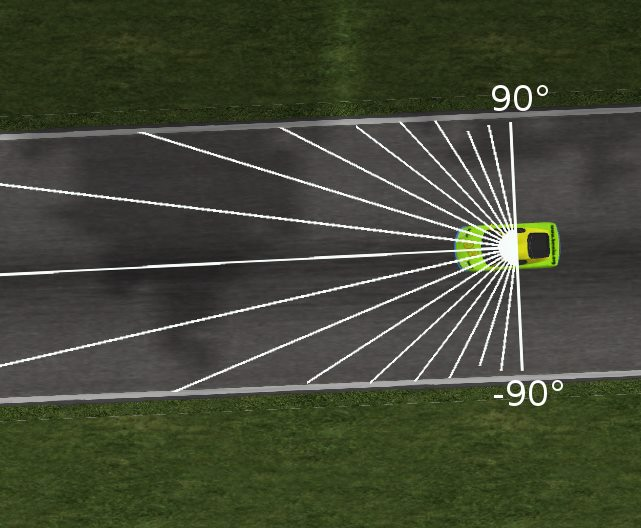
\includegraphics[width=\textwidth]{img/FSM5Sensors}
   \caption{Range finders configuration.}\label{fig:FSMDriver5Finders}%
\end{subfigure}
   \caption{FSMDriver5 model.}\label{fig:FSMDriver5}
\end{figure*}

Initial tests showed that transitioning from \SL~to \C~was too swift, hampering performance because the car consistently entered curves at such high speeds that the controller was unable to turn and exited the track, so the additional behavior \AC~was implemented.

\AC~positions the driver towards the outside of the incoming curve and tries to race at a speed proportional to the curvature, so less braking would be necessary in \C. Thus, a 5-state FSMDriver model (FSMDriver5, illustrated in Figure~\ref{fig:FSMDriver5Model}) was ready for testing. The range sensors were arbitrarily configured at every $10$ degrees from $-90$ to $90$ relative to the car's front axis (that is, a uniform distribution from the left to the right of the car), as shown in Figure~\ref{fig:FSMDriver5Finders}.

Sensor readings provide an the controller's perception of the car's position of location in the track and, since \SL~ aims to drive parallel to the central axis of the track, the changes in how the range finders' input are spread out around their mean value can be used to switch between states because the difference between frontal and lateral sensors is larger when driving in a straight line than in a curve. This variance of the readings is computed as follows:

\begin{equation}
	variance = \frac{1}{19}\sum_{i=1}^{19}[(RF_i-\mu)^2]
\end{equation}

\noindent
where $RF_i$ is the input from the $i$-th range finder and $\mu$ is the mean value of all such readings. The resulting value is considered in the transition function to define the current state of the \racing~behavior, as described in Algorithm~\ref{alg:FSMDriver5}.

\begin{algorithm}[h]%
\caption{FSMDriver5 Transition}%
\label{alg:FSMDriver5}%
\begin{algorithmic}
    \IF{car is stuck}
        \STATE $state \Leftarrow \St$
    \ELSE
		\IF{$variance$ is in \SL~thresholds \AND
		the current state is not \SL}
			\STATE $state \Leftarrow \SL$
		\ELSIF{$variance$ is not in \AC~thresholds \AND
		current state is not \C}
			\STATE $state \Leftarrow \AC$
		\ELSIF{$variance$ is in \AC~thresholds \AND
		current state is not \AC}
			\STATE $state \Leftarrow \AC$
		\ELSIF{$variance > 0$}
			\STATE $state \Leftarrow \C$
		\ELSE
			\STATE $state \Leftarrow \OT$
		\ENDIF
	\ENDIF
\end{algorithmic}
\end{algorithm}

After several iterations adjusting the configurations, this model also had an acceptable performance. However, testing also revealed that the transitions between states required were the bottleneck for improved racing. Not only some of the triggers needed a more detailed analysis to avoid eventual erratic behavior, but the sheer number parameters considered for transitioning, each with its triggers (see Figure~\ref{fig:FSMDriver5Model}), and their impact on the model's behavior during a complete race caused the whole model to be thought over.

Analyzing FSMDriver5's transitions occurrences within a race, it was clear that the \recovery~behavior had two distinct situations, which were acceptably handled by the current configuration, and that the major issue was frequent triggering between the \racing~states, which inevitably resulted in the car leaving the track and jeopardizing its performance.



%%%%%%%%%%%%%%%%%%%%%%%%%%%%%%%%%%%%%%%%%%%%%%%%%%%%%%%%%%%%%%%%%%%%%%%%%%%%%%%%
%%%%%%%%%%%%%%%%%%%%%%%%%%%%%%%%%%%%%%%%%%%%%%%%%%%%%%%%%%%%%%%%%%%%%%%%%%%%%%%%
%%%%%%%%%%%%%%%%%%%%%%%%%%%%%%%%%%%%%%%%%%%%%%%%%%%%%%%%%%%%%%%%%%%%%%%%%%%%%%%%



\subsection{FSMDriver3}%
To reduce the model's complexity, and considering the intuitive division of behaviors proposed, a new model where the defined \recovery~behaviors were maintained and the \racing~behaviors were joined into a new state called \IT. Figure~\ref{fig:FSMDriver3Model} illustrates this FSMDriver3 model.

\begin{figure*}
\centering
\begin{subfigure}[b]{0.4\textwidth}
   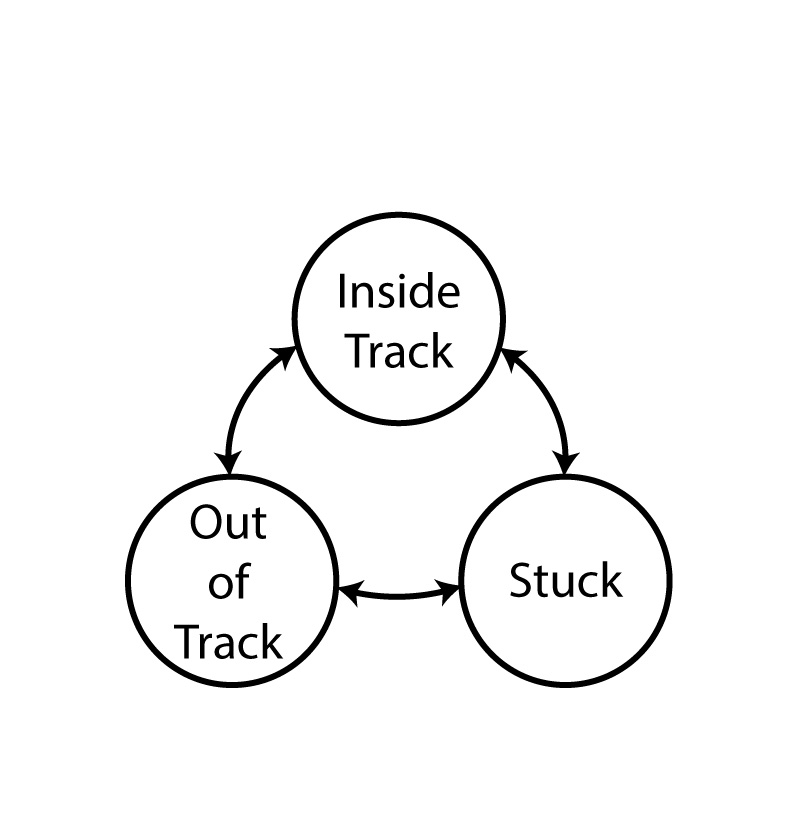
\includegraphics[width=\textwidth]{img/ThreeStateFSM}
   \caption{States and transitions.}\label{fig:FSMDriver3Model}%
\end{subfigure}
\begin{subfigure}[b]{0.4\textwidth}
   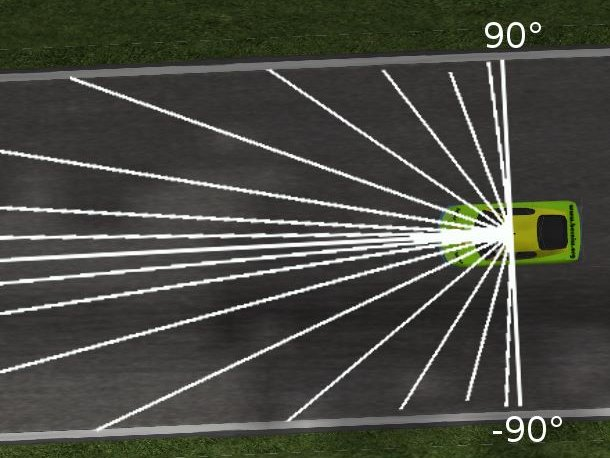
\includegraphics[width=\textwidth]{img/FSM3Sensors}
   \caption{Range finders configuration.}\label{fig:FSMDriver3Finders}%
\end{subfigure}
   \caption{FSMDriver3 model.}\label{fig:FSMDriver3}
\end{figure*}

\recovery, though essential for championship disputes, rarely occurred after FSMDriver5 the accepted initial configuration (through trial and error). The new \racing~state implements a very straightforward idea, accelerate to an arbitrary target speed towards the largest open space inside track limits, including both the straight and the curved portions of the track. The target speed is proportional to the largest sensor reading, and braking is activated if the current speed is greater than the target speed. Gear changing works based on RPM threshold as in FSMDriver5.

In order to have more detailed information on track segment straight ahead, which will guide the movement, more range finders are placed in front of the car in a uniform distribution (as shown in Figure~\ref{fig:FSMDriver3Finders}), contrasting with FSMDriver5's equidistant placement. This different approach to driving lead to a reimplementation of the transition function, as shown in Algorithm~\ref{alg:FSMDriver3}:

\begin{algorithm}[h]%
\caption{FSMDriver3 Transition}%
\label{alg:FSMDriver3}%
\begin{algorithmic}
    \IF{car is stuck}
        \STATE $state \Leftarrow \St$
    \ELSE
        \IF{car is within track limits}
            \STATE $state \Leftarrow \IT$
        \ELSE
            \STATE $state \Leftarrow \OT$
        \ENDIF
    \ENDIF
\end{algorithmic}
\end{algorithm}

The new transition dismisses the computation of the variance and is clearly more intuitive. Initially, configurations resembling FSMDriver5's parameters were set and manually adjusted until a behavior similar to the original driver was achieved. As expected, this process was quicker than for FSMDriver5 and soon a configuration better than some robots was available.

Considering both FSMDriver3 and FSMDriver5 models as acceptable drivers, the next step is to define proper configurations as to have them behave acceptably as racing controllers, maximizing their performance in the TORCS/SCR environment.



%%%%%%%%%%%%%%%%%%%%%%%%%%%%%%%%%%%%%%%%%%%%%%%%%%%%%%%%%%%%%%%%%%%%%%%%%%%%%%%%
%%%%%%%%%%%%%%%%%%%%%%%%%%%%%%%%%%%%%%%%%%%%%%%%%%%%%%%%%%%%%%%%%%%%%%%%%%%%%%%%
%%%%%%%%%%%%%%%%%%%%%%%%%%%%%%%%%%%%%%%%%%%%%%%%%%%%%%%%%%%%%%%%%%%%%%%%%%%%%%%%



\subsection{Offline Learning: Evolving Parameters}%
To search for an optimal solution, a genetic algorithm was selected between possible techniques not only due to its successful application in similar (and very different) problems, but also because of its more general nature: only a representation of a solution and a means to measuring its quality must be specifically defined for the task. Considering the evolution of the drivers' parameters, a solution (or an individual) was represented by a string of bits, which compose the floating point parameters of the FSMDrivers' models.

FSMDriver5 has, overall, 22 parameters that need to be specified in the transition function and states. The function considers 4 threshold values defining 2 intervals, one for identifying the variance levels for \SL~and another for \AC. \SL~also considers 4 threshold values, one for a minimal racing gear, and 3 for identifying RPM values that indicate when to increase/decrease gear.

\AC~has 3 parameters: a desired position to enter the upcoming curve (in relation to the track axis), a lower speed threshold, and a maximum steering value. \OT considers 7 parameters: two angle thresholds defining an acceptable angle interval for returning to the track, 3 speed thresholds for changing gears, a maximum breaking threshold to avoid skidding, and decelerating intensity to reduce the speed before entering the curve.

\St~has 4 parameters, one for defining a starting distance before considering the car stuck, one for tracking the current speed to determine if it is still stuck, and two for defining game ticks thresholds, establishing an amount of time to consider before triggering a transition to this state.

FSMDriver3, on the other hand, has the same 11 for \OT~and \St~as FSMDriver5, and 6 additional for \IT. There is one for a minimal racing gear, 3 for identifying RPM values to increase/decrease gear, one for defining a ratio between car speed and range finder reading for setting the target speed, and a base speed value to control brake and acceleration actuators.

The solution is then modeled as a string of enough bits to represent each floating point value for as many parameters as necessary, according to the model. The GA also requires a fitness function to evaluate the solutions, the same for either model. There are several possibilities (damage taken, similarity to a human driver, etc.), but his work will focus on the standard metric for SCR: the distance raced during a fixed time period.



%%%%%%%%%%%%%%%%%%%%%%%%%%%%%%%%%%%%%%%%%%%%%%%%%%%%%%%%%%%%%%%%%%%%%%%%%%%%%%%%
%%%%%%%%%%%%%%%%%%%%%%%%%%%%%%%%%%%%%%%%%%%%%%%%%%%%%%%%%%%%%%%%%%%%%%%%%%%%%%%%
%%%%%%%%%%%%%%%%%%%%%%%%%%%%%%%%%%%%%%%%%%%%%%%%%%%%%%%%%%%%%%%%%%%%%%%%%%%%%%%%



\subsection{Online Learning: Staying in Track}%
An online learning module was included in FSMDriver3 trying to improve its performance, in an attempt to reduce damage and time loss for racing out of the track. Whenever the driver enters \OT, the speed and location of this occurrence are recorded and used in the \racing~state. If the speed is over a threshold, the model assumes the driver has left the track due to excessive speed and uses this information to slow down the driver in subsequent laps when approaching the recorded places, trying to remain inside the track.

This behavior does not interfere with the breaking actions in the model, but does affect the driver's performance and, thus, with the offline learning process. Though any controller can also learn where it leaves the track (if so), the differences in implementation of the \racing~states in the FSMDrivers considered here are such that slowing down before the recorded places implies on excessive additional complexity in FSMDriver5 and, therefore, this learning module was not implemented for this controller.